\documentclass[tikz,border=8pt]{standalone}
% Shared look for every TikZ diagram. Load with \input{../../tools/tikz-style.tex}
\usepackage[T1]{fontenc}
\usepackage{lmodern}
\renewcommand{\sfdefault}{lmr}  % diagrams use the same serif as the text
\usetikzlibrary{arrows.meta, positioning, shapes.geometric, calc, fit, backgrounds}
\definecolor{cblue}{HTML}{4C78A8}
\definecolor{corange}{HTML}{F58518}
\definecolor{cgreen}{HTML}{54A24B}
\definecolor{cred}{HTML}{E45756}
\definecolor{cpurple}{HTML}{B279A2}
\definecolor{cgrey}{HTML}{6B6B6B}
\tikzset{
  every picture/.style={font=\sffamily, line width=1.2pt},
  box/.style={draw=#1, fill=#1!12, rounded corners=4pt, align=center, inner sep=7pt, minimum height=1.1cm},
  box/.default=cgrey,
  arrow/.style={-{Stealth[length=3mm]}, draw=cgrey, line width=1.4pt},
  title/.style={font=\sffamily\bfseries\Large},
  note/.style={font=\sffamily\small, text=cgrey, align=center},
}
\AtBeginDocument{\hyphenpenalty=10000 \exhyphenpenalty=10000}

\begin{document}
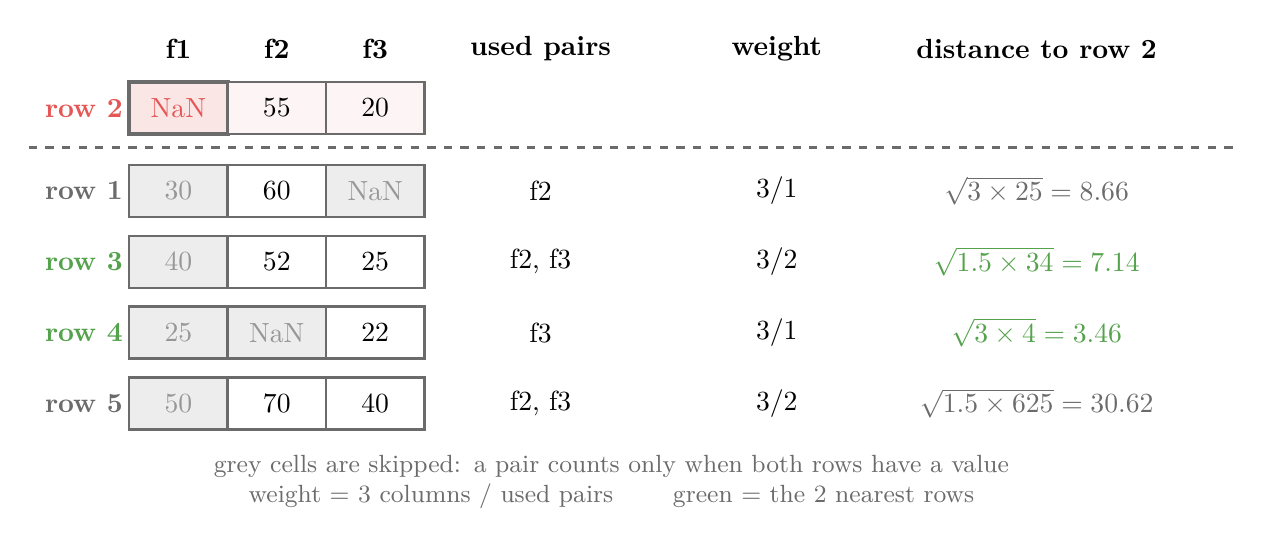
\begin{tikzpicture}[cell/.style={draw=cgrey, line width=0.8pt, minimum width=1.25cm, minimum height=0.66cm, font=\sffamily},
                    off/.style={cell, fill=cgrey!12, text=cgrey!70}]
  \def\dy{0.9}
  % header
  \foreach \c/\h in {0/f1, 1/f2, 2/f3} \node[font=\sffamily\bfseries] at (1.25*\c,0.75) {\h};
  \node[font=\sffamily\bfseries] at (4.6,0.75) {used pairs};
  \node[font=\sffamily\bfseries] at (7.6,0.75) {weight};
  \node[font=\sffamily\bfseries] at (10.9,0.75) {distance to row 2};
  % row 2
  \node[font=\sffamily\bfseries, text=cred] at (-1.2,0) {row 2};
  \node[cell, fill=cred!15, text=cred, line width=1.4pt] at (0,0) {NaN};
  \node[cell, fill=cred!6] at (1.25,0) {55};
  \node[cell, fill=cred!6] at (2.5,0) {20};
  \draw[cgrey, line width=0.8pt, dashed] (-1.9,-0.5) -- (13.4,-0.5);
  % other rows: f1 is never used (row 2 lacks it)
  \foreach \r/\a/\b/\cc/\ob/\oc/\pairs/\w/\d/\col [count=\i] in {
      1/30/60/NaN/0/1/{f2}/{3/1}/{$\sqrt{3 \times 25} = 8.66$}/cgrey,
      3/40/52/25/0/0/{f2, f3}/{3/2}/{$\sqrt{1.5 \times 34} = 7.14$}/cgreen,
      4/25/NaN/22/1/0/{f3}/{3/1}/{$\sqrt{3 \times 4} = 3.46$}/cgreen,
      5/50/70/40/0/0/{f2, f3}/{3/2}/{$\sqrt{1.5 \times 625} = 30.62$}/cgrey} {
    \pgfmathsetmacro{\y}{-\dy*\i-0.15}
    \node[font=\sffamily\bfseries, text=\col] at (-1.2,\y) {row \r};
    \node[off] at (0,\y) {\a};
    \ifnum\ob=1 \node[off] at (1.25,\y) {\b}; \else \node[cell] at (1.25,\y) {\b}; \fi
    \ifnum\oc=1 \node[off] at (2.5,\y) {\cc}; \else \node[cell] at (2.5,\y) {\cc}; \fi
    \node at (4.6,\y) {\pairs};
    \node at (7.6,\y) {$\w$};
    \node[text=\col, font=\sffamily\bfseries] at (10.9,\y) {\d};
  }
  \node[note, text width=13cm] at (5.5,-4.75) {grey cells are skipped: a pair counts only when both rows have a value\\ weight = 3 columns / used pairs \qquad green = the 2 nearest rows};
\end{tikzpicture}
\end{document}
